\section{Communication delay project}
This project ~\cite{Nguyen:2008:ICGSE} used data we mined as described in this
paper and we describe it as an illustration of our
design principles and conducting research using software development artifacts.

There were two main objectives of this project: (1) to examine if the Jazz team
experience communication and task completion delay due to the large geographic
distance between the teams and (2) gain insights about communication patterns of
the entire project team. For the first objective, we conceptualized communication
delay as the difference between comments on work items and task completion delay
by the resolution time of a work item. Thus, we had to query all work items from
the Jazz repository. With the information on work items we addressed our second
objective by constructing and examining a project-wide communication-based
social network that connecting developers that commented on the same work items.

\begin{figure}[t]
	\begin{center}
	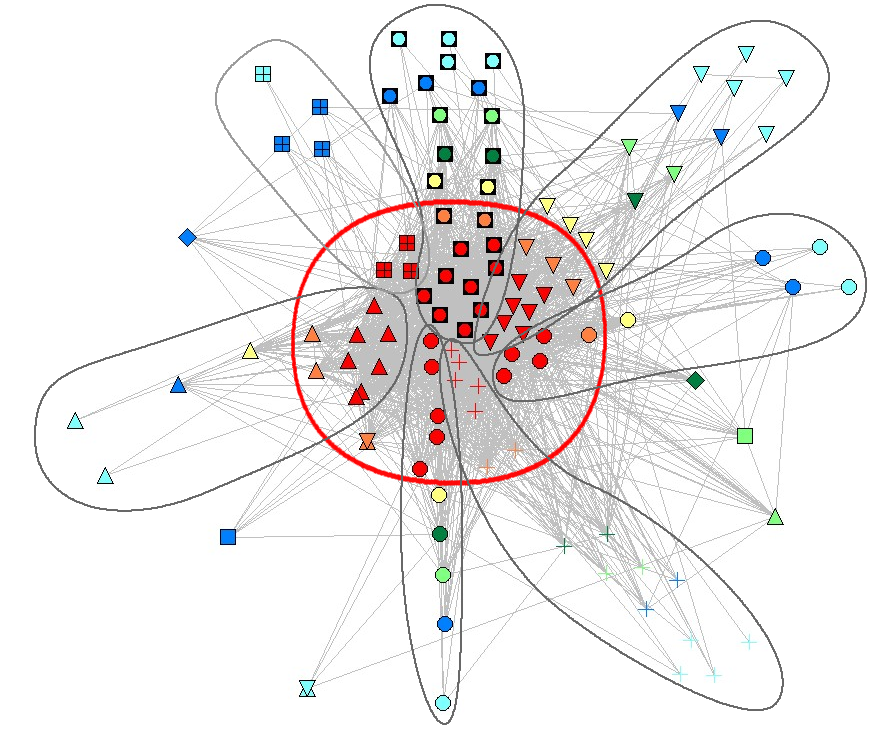
\includegraphics[width=.99\columnwidth]{./Figures/Figure03SocialNetwork}
	\caption{The communication based social network of the Jazz development team}
	\label{fig:SocialNetwork}
	\end{center}
\end{figure}

Following an iterative process, we first designed a query for a teams' hierarchy.
Subsequently, we wrote a query to retrieve the members of each team. In
the next iteration we designed the query to retrieve all work items. This query
induced a high load on the repository due to the large amount of data that was
contained in all work items. During the early versions of Jazz we encountered
client and server side failures cause by our query. To minimize the additional
load generated from re-running a crashed query, our tool stores a cache of the
queried data which does not need to be extracted during the re-run. When it is
resumed, the query picks up from where it left. We were able to extend the tool
and extract the data within the first six months of our project.

With the information from the work items, our analysis suggests that
the Jazz team did not experience as much delay as reported in previous
literatures~\cite{Battin:2001tb,Herbsleb:2003oo}. We hypothesize that this is due
to the new integrated development support provided by Jazz as well as advances
in software practices used by the Jazz distributed team.

Using this data we also constructed the project-wide social network based on communication as shown in Figure~\ref{fig:SocialNetwork}. The shape of the nodes (and the flower-like petals) indicate the developers' geographical location. The color of the nodes indicate how active each developers is in the overall network from most active (red) to least active (light blue). The red circle emphasizes the active core members of the project.